\documentclass[10pt]{beamer}
\usepackage[utf8]{inputenc}
\usepackage[spanish]{babel}
\usepackage{tikz}
\usepackage{xcolor}
\usepackage{graphicx}
\usepackage{amsmath}
\usepackage{amssymb}
\usepackage{multirow}
\usepackage{caption}
\usepackage{makecell}
\usepackage{multirow}
\usepackage{array}
\usepackage{esint}
\usepackage{adjustbox}
\usepackage{tabularht}
\usepackage{float}
\usepackage{hyperref}
\usepackage{nicefrac}    
\usepackage{microtype}
\usepackage{booktabs}
\usepackage{url}

\usetheme{sleep-states}
\usefonttheme[onlymath]{serif}



\title{\Huge{A Deep Learning approach to detect sleep states}}
\author{Armando Bringas, Alexis Guerrero}
\date{3rd January - 2024}




\begin{document}

\begin{frame}
  \titlepage
\end{frame}

\begin{frame}
  \frametitle{Introduction}
  \begin{block}{}
    Lorem ipsum dolor sit amet, consectetur adipiscing elit, sed do eiusmod tempor incididunt ut labore et dolore magna aliqua. Ut enim ad minim veniam, quis nostrud exercitation ullamco laboris nisi ut aliquip ex ea commodo consequat. Duis aute irure dolor in reprehenderit in voluptate velit esse cillum dolore eu fugiat nulla pariatur. Excepteur sint occaecat cupidatat non proident, sunt in culpa qui officia deserunt mollit anim id est laborum
  \end{block} 
\end{frame}

\begin{frame}
  \frametitle{Literature Review}
  \begin{block}{}
    Lorem ipsum dolor sit amet, consectetur adipiscing elit, sed do eiusmod tempor incididunt ut labore et dolore magna aliqua. Ut enim ad minim veniam, quis nostrud exercitation ullamco laboris nisi ut aliquip ex ea commodo consequat. Duis aute irure dolor in reprehenderit in voluptate velit esse cillum dolore eu fugiat nulla pariatur. Excepteur sint occaecat cupidatat non proident, sunt in culpa qui officia deserunt mollit anim id est laborum
  \end{block} 
\end{frame}

\begin{frame}
  \frametitle{Dataset}
  \begin{block}{}
    Dataset consists of approximately 500 multi-day recordings from wrist-mounted accelerometers. The accelerometer data in the dataset was processed using R with the GGIR package \cite{Migueles2019GGIR}. The recordings are labeled with two event types: 'onset', indicating the start of sleep, and 'wakeup', marking its end. The primary objective is to identify these two events within the accelerometer data series, this primarily represents a binary classification task. 
    \begin{figure*}
        \centering
        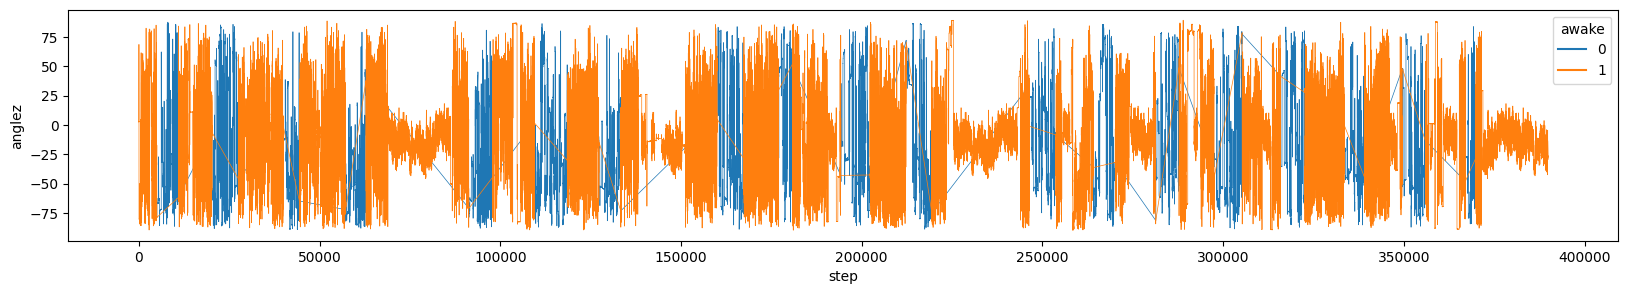
\includegraphics[width=1\linewidth]{038441c925bb_anglez.png}
        \caption{Accelerometer training data. Plot of \texttt{step} againts \texttt{anglez} showing \texttt{event} state}
        \label{fig:accelerometerdata_series-038441c925bb_anglez}
    \end{figure*}
  \end{block} 
\end{frame}

\begin{frame}
  \frametitle{Model - Random Forest}
  \begin{block}{}
    Lorem ipsum dolor sit amet, consectetur adipiscing elit, sed do eiusmod tempor incididunt ut labore et dolore magna aliqua. Ut enim ad minim veniam, quis nostrud exercitation ullamco laboris nisi ut aliquip ex ea commodo consequat. Duis aute irure dolor in reprehenderit in voluptate velit esse cillum dolore eu fugiat nulla pariatur. Excepteur sint occaecat cupidatat non proident, sunt in culpa qui officia deserunt mollit anim id est laborum
  \end{block} 
\end{frame}

\begin{frame}
  \frametitle{Model - LSTM}
  \begin{block}

        We are proposing a starting neural network architecture with the following blocks where consists of an LSTM layer of 64 units, ideal for processing sequences by capturing dependencies from prior inputs. This is followed by a Dense layer, the size of which matches the number of classification categories in your problem, in this case for our binary classification problem \(n_{\text{classes}} = 2\). The final component is a softmax activation function, applied to convert the output into a probability distribution across the predicted classes. 
        \begin{figure}[h]
          \centering
          \[
          \xrightarrow{\text{input}} \boxed{\text{LSTM} (64)} \rightarrow \boxed{\text{Dense} (n_{\text{classes}})} \xrightarrow{\text{softmax}}
          \]
          \caption{Neural Network for accelerometer data classification}
          \label{fig:neuralnetwork}
        \end{figure}
  \end{block} 
\end{frame}

\begin{frame}
  \frametitle{Evaluation Metrics}
  \begin{block}{}
    Lorem ipsum dolor sit amet, consectetur adipiscing elit, sed do eiusmod tempor incididunt ut labore et dolore magna aliqua. Ut enim ad minim veniam, quis nostrud exercitation ullamco laboris nisi ut aliquip ex ea commodo consequat. Duis aute irure dolor in reprehenderit in voluptate velit esse cillum dolore eu fugiat nulla pariatur. Excepteur sint occaecat cupidatat non proident, sunt in culpa qui officia deserunt mollit anim id est laborum
  \end{block} 
\end{frame}

\begin{frame}
  \frametitle{Results}
  \begin{block}{}
    Lorem ipsum dolor sit amet, consectetur adipiscing elit, sed do eiusmod tempor incididunt ut labore et dolore magna aliqua. Ut enim ad minim veniam, quis nostrud exercitation ullamco laboris nisi ut aliquip ex ea commodo consequat. Duis aute irure dolor in reprehenderit in voluptate velit esse cillum dolore eu fugiat nulla pariatur. Excepteur sint occaecat cupidatat non proident, sunt in culpa qui officia deserunt mollit anim id est laborum
  \end{block} 
\end{frame}


\begin{frame}
  \frametitle{Conclusion}
  \begin{block}{}
    Lorem ipsum dolor sit amet, consectetur adipiscing elit, sed do eiusmod tempor incididunt ut labore et dolore magna aliqua. Ut enim ad minim veniam, quis nostrud exercitation ullamco laboris nisi ut aliquip ex ea commodo consequat. Duis aute irure dolor in reprehenderit in voluptate velit esse cillum dolore eu fugiat nulla pariatur. Excepteur sint occaecat cupidatat non proident, sunt in culpa qui officia deserunt mollit anim id est laborum
  \end{block} 
\end{frame}


\begin{frame}
  \frametitle{Bibliography}
  \begin{block}{}
    {
        \small
        %%%%%%%%%%%%%
        \bibliographystyle{plainnat} % or another suitable style
        \bibliography{bibliography} % replace with your BibTeX file name
    }
  \end{block} 
\end{frame}

\end{document}
